\RequirePackage[T1]{fontenc}
\documentclass[10pt,conference,compsocconf]{IEEEtran}
\usepackage{amsmath,booktabs,graphicx}
\usepackage[hidelinks]{hyperref}
\linespread{1.00}
% Generated from report/audit/current_results.json; do not edit values by hand.
\newcommand{\SelectedThreshold}{0.185}
\newcommand{\HoldFone}{0.4385}
\newcommand{\HoldAccuracy}{0.8667}
\newcommand{\HoldPrecision}{0.3491}
\newcommand{\HoldRecall}{0.5894}
\newcommand{\FitMissing}{44.79}
\newcommand{\RawFeatures}{185}
\newcommand{\CompactDim}{187}
\newcommand{\BroadDim}{643}
\newcommand{\InteractionDim}{702}
\newcommand{\FinalDim}{645}
\newcommand{\MajorityAccuracy}{0.9117}
\newcommand{\DefaultFone}{0.2237}
\newcommand{\DefaultAccuracy}{0.9133}
\newcommand{\ThresholdGain}{0.2148}
\newcommand{\TruePositive}{1,708}
\newcommand{\HoldPositive}{2,898}
\newcommand{\FalsePositive}{3,185}
\newcommand{\FalseNegative}{1,190}
\newcommand{\TuneFone}{0.4245}
\newcommand{\TuningRows}{Compact & $10^{-5}$ & 0.185 & 0.4210 & 0.8638 \\
Compact & $10^{-4}$ & 0.185 & 0.4195 & 0.8643 \\
Compact & $10^{-3}$ & 0.175 & 0.4145 & 0.8592 \\
Broad & $10^{-5}$ & 0.170 & 0.4234 & 0.8556 \\
\textbf{Broad} & $10^{-4}$ & 0.185 & 0.4245 & 0.8642 \\
Broad & $10^{-3}$ & 0.180 & 0.4204 & 0.8612 \\
Interactions & $10^{-5}$ & 0.185 & 0.4232 & 0.8620 \\
Interactions & $10^{-4}$ & 0.195 & 0.4239 & 0.8672 \\
Interactions & $10^{-3}$ & 0.185 & 0.4202 & 0.8623 \\}
\newcommand{\AblationText}{The tuning results in Table~\ref{tab:tuning} favor Broad features with $\lambda=10^{-4}$ and threshold 0.185. At fixed $\lambda=10^{-4}$, expanding Compact to Broad raises tuning F1 from 0.4195 to 0.4245, a gain of 0.0050. Adding interactions gives 0.4239; Broad has the highest tuning F1 among the nine candidates. Each candidate uses its own threshold selected by the same rule. The gain from additional survey fields is larger than the difference between Broad and Interactions.}

\begin{document}
\title{Heart Disease Classification with Categorical Features and Threshold Selection}
\author{Boyang Hu, Jinrun Jiang, Yunqing Pan\\\textit{Equal contribution; authors listed alphabetically by surname.}\\CS-433 Machine Learning, EPFL -- Fall 2026}
\maketitle
\begin{abstract}
We use logistic regression implemented in NumPy to classify reported heart disease from 321 survey features. The dataset contains 328,135 labeled respondents, with 8.83\% positive labels. We compare three feature sets and three regularization strengths, selecting the model and decision threshold on a separate tuning set. The selected model uses a broad set of categorical and numeric features with regularization $\lambda=10^{-4}$. At threshold \SelectedThreshold{}, it achieves F1 \HoldFone{} and accuracy \HoldAccuracy{} on 32,814 holdout respondents. The broader feature set gives the highest tuning F1. A threshold below 0.5 increases holdout F1 by identifying more positive cases, with more false positive predictions.
\end{abstract}

\section{Task and evaluation design}
The project predicts the binary \texttt{\_MICHD} label from the supplied BRFSS survey data. A positive label indicates that the respondent reported a diagnosis of coronary heart disease or a heart attack. There are 28,975 positive labels among the 328,135 labeled rows.

Class imbalance makes accuracy an incomplete measure: predicting every respondent as negative gives about 91.17\% accuracy but finds no positive cases. We therefore select models by positive-class F1 and report accuracy alongside it. With true positives $TP$, false positives $FP$, false negatives $FN$ and true negatives $TN$, the metrics are
\[
F1=\frac{2TP}{2TP+FP+FN},\qquad
\mathrm{accuracy}=\frac{TP+TN}{n}.
\]


We set the NumPy random seed to 42, shuffle rows within each class, and assign 75\% to fitting, 15\% to tuning and 10\% to holdout evaluation. This gives 246,101, 49,220 and 32,814 rows, respectively. We learn preprocessing rules and model weights from the fitting set. We use the tuning set to select the feature set, regularization strength and classification threshold. We then evaluate the selected configuration on the holdout set.

\section{Methods}
\subsection{Cleaning and encoding survey responses}
In the fitting set, \FitMissing{}\% of feature entries are missing. We exclude the first 26 survey fields, the block from \texttt{QSTVER} through \texttt{\_LLCPWT}, and the rehabilitation questions \texttt{HAREHAB1} and \texttt{STREHAB1}. These exclusions remove survey administration and household fields, sampling weights and post-event questions. The heart rehabilitation question directly refers to a previous heart attack. We retain other fields if more than 10\% of fitting values are non-missing and they include at least two distinct values.

For the health-day counts \texttt{PHYSHLTH}, \texttt{MENTHLTH} and \texttt{POORHLTH}, code 88 means no days and is replaced by zero. Codes 77/99 indicate unknown or refused answers and are treated as missing. For weekly drinking \texttt{\_DRNKWEK}, code 99900 is also treated as missing. Other response codes are kept as recorded.

We treat fields with at most 16 distinct non-missing values as categorical. Each category gets a 0/1 column, except the most frequent category, which serves as the baseline. Missing responses and categories not seen during fitting have zeros in these category columns. For fields with more than 16 distinct values, we fill missing entries with the fitting median. We limit values to the fitting 1st--99th percentile interval, subtract the median and divide by the interval width, using a minimum divisor of one. Each field also gets a 0/1 column marking missing entries. We remove constant columns but keep the intercept. All rules are learned from the fitting set and reused for tuning and holdout data.

\subsection{Three feature sets}
The \emph{Compact} set uses 48 predefined fields covering age, sex, general health, diagnosed conditions, physical limitations and lifestyle. The notebook lists these fields in \texttt{CORE}. The \emph{Broad} set uses all \RawFeatures{} fields that pass filtering. Both sets use the same encoding rules. The \emph{Interactions} set extends Broad with 0/1 columns for combinations of age and sex, age and general health, and sex and general health. Age is grouped into 18--27, 28--37, $\ldots$, 68--77 and 78+; sex uses codes 1/2 and general health uses codes 1--5. These combinations add 59 columns before constant-column removal. The resulting fitting matrices contain \CompactDim{}, \BroadDim{} and \InteractionDim{} columns, respectively, including the intercept.

\subsection{Logistic regression and model selection}
For an encoded row $x_i$, logistic regression estimates the probability of a positive label as $p_i=1/(1+\exp(-x_i^\top w))$. We minimize
\[
\frac{1}{n}\sum_{i=1}^{n}\left[\log(1+e^{x_i^\top w})-y_i x_i^\top w\right]
+\lambda\sum_{j=1}^{d-1}w_j^2,
\]
Here, $n$ is the number of fitting rows, $d$ is the number of columns including the intercept, and $w_0$ is the unpenalized intercept. The L2 penalty discourages large feature weights. We initialize the intercept to the log-odds of the fitting positive rate and all other weights to zero.

We fit the model with L-BFGS, which uses recent weight and gradient changes to choose an update direction. We keep ten such pairs and allow at most 200 updates, stopping when the largest absolute gradient is below $2\times10^{-5}$. For each update, we try at most 20 step sizes, starting at one and halving until the loss decreases enough to meet the Armijo condition with coefficient $10^{-4}$. Training stops if no step is accepted. Feature matrices and matrix products use float32; weights and optimizer updates use float64. The loss uses \texttt{logaddexp} for numerical stability.

Each feature set is tested with $\lambda\in\{10^{-5},10^{-4},10^{-3}\}$, giving nine candidates. For each one, we test thresholds $0.10,0.105,\ldots,0.40$ and $0.50$. We predict a positive label when $p_i$ is at least the threshold. We select the threshold with the highest tuning F1; ties are resolved by higher accuracy and then a higher threshold. We select the model by tuning F1, using accuracy to resolve ties.

The separate \texttt{implementations.py} module supplies the six required course methods: linear regression by full-batch gradient descent, single-row SGD and normal equations; ridge regression; and logistic regression with and without L2 regularization. Linear loss is $\|y-Xw\|^2/(2n)$; ridge solves $(X^\top X+2n\lambda I)w=X^\top y$. Each function returns final weights and unpenalized mean loss. The experiments below use the notebook's logistic optimizer.

\section{Results and interpretation}
\begin{table}[t]
\centering
\caption{Tuning results for all nine candidates. Each candidate uses the threshold $t$ with the highest tuning F1. Bold marks the selected model.}
\label{tab:tuning}
\small
\begin{tabular}{llrrr}
\toprule
Features & $\lambda$ & $t$ & F1 & Accuracy\\
\midrule
\TuningRows
\bottomrule
\end{tabular}
\end{table}

\AblationText{}

\begin{table}[t]
\centering
\caption{Holdout results on 32,814 rows. Both logistic rows use the same fitted weights.}
\label{tab:holdout}
\small
\begin{tabular}{lrr}
\toprule
Decision rule & F1 & Accuracy\\
\midrule
Always negative & 0.0000 & \MajorityAccuracy{}\\
Selected model, $t=0.500$ & \DefaultFone{} & \DefaultAccuracy{}\\
Selected model, $t=\SelectedThreshold{}$ & \HoldFone{} & \HoldAccuracy{}\\
\bottomrule
\end{tabular}
\end{table}

\newpage
Table~\ref{tab:holdout} compares two thresholds using the same model weights. Changing it from 0.5 to \SelectedThreshold{} raises holdout F1 by \ThresholdGain{}. At the selected threshold, the model finds \TruePositive{} of \HoldPositive{} positive cases, giving recall \HoldRecall{}. Of its positive predictions, a fraction \HoldPrecision{} are correct (precision). It produces \FalsePositive{} false positives and misses \FalseNegative{} positive cases.

\begin{figure}[t]
\centering
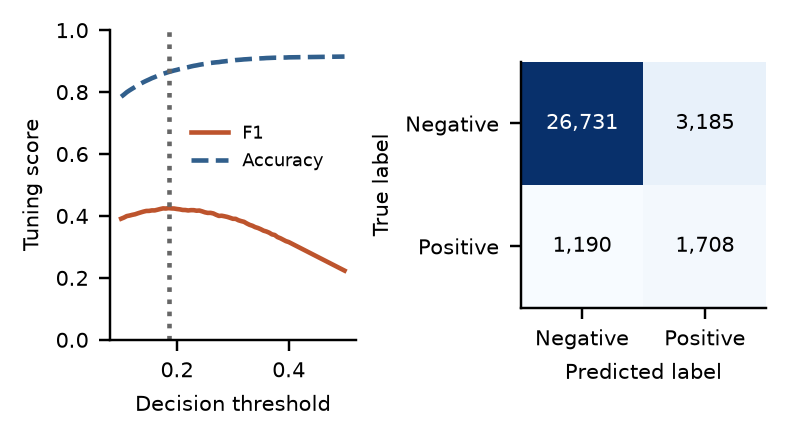
\includegraphics[width=\columnwidth]{../figures/evaluation.png}
\caption{Left: tuning F1 and accuracy across decision thresholds; the dotted line marks the selected threshold. Right: holdout confusion counts for that model and threshold.}
\label{fig:eval}
\end{figure}

Figure~\ref{fig:eval} shows the tuning scores across thresholds and the holdout confusion counts. The selected model has tuning F1 \TuneFone{} and holdout F1 \HoldFone{}.

\section{Final model and conclusion}
After holdout evaluation, we learn the preprocessing rules again using all 328,135 labeled rows and refit the selected Broad model with $\lambda=10^{-4}$. The final design has \FinalDim{} columns including the intercept. The tuning-selected threshold \SelectedThreshold{} is kept for the 109,379 unlabeled rows. The output \texttt{submission.csv} preserves their original IDs and order and uses labels $-1/+1$. The reported run uses Python 3.13.15 and NumPy 2.5.2. The notebook contains the full training and export workflow; \texttt{results/model.npz} stores the final weights and threshold.

Broad features give higher tuning F1 than the compact baseline. Selecting the threshold raises holdout F1 from \DefaultFone{} to \HoldFone{}, with accuracy \HoldAccuracy{}. These results support using both survey feature selection and threshold tuning for this task.

\end{document}
